\documentclass{beamer}
\usecolortheme{wolverine}

% math stuff
\usepackage{amsmath}
\usepackage{amsthm}
\usepackage{amssymb}
\usepackage{xcolor}

\usepackage{float}
\usepackage{subcaption}

% to insert images
\usepackage{graphicx}

% to correctly insert stressed characters
\usepackage[T1]{fontenc}
\usepackage[utf8]{inputenc}

\usepackage{multirow}

% Bibliography
\usepackage[style=alphabetic]{biblatex}
% \usepackage[nottoc]{tocbibind}
\usepackage{bibentry}
\setcounter{biburllcpenalty}{9000}
\usepackage{nameref}
\addbibresource{slides.bib}

% to put links in table of contents
\usepackage{hyperref}
\hypersetup{colorlinks=false, %set true if you want colored links
	linktoc=all,     %set to all if you
}

\usepackage{mathtools}

% Add symbols
% \usepackage{textcomp}

% Add command for Real and Z sets
% \usepackage{dsfont}
% \newcommand{\Rset}{$\mathds{R}$}
% \newcommand{\Zset}{$\mathds{Z}$}

% Code highlighting
% \usepackage{minted}
% \usemintedstyle{perldoc}
% \setminted{
%     frame=single,
%     breaklines,
% }

% tikz figures
% \usepackage{tikz}
% \input{style.tikzstyle}
% \usetikzlibrary{positioning}

% number rounding
\usepackage{siunitx}
\sisetup{round-mode=places,round-precision=5}

\definecolor{myyellow}{RGB}{225, 225, 0}

\title{Thesis notes}
\date{30th March}

% any code between @(...)@ is escaped back to LaTeX
% \lstset{escapeinside={@(}{)@}}

% algorithms
\usepackage[ruled,vlined]{algorithm2e}

\begin{document}
\frame{\titlepage}

\begin{frame}[c]
	\frametitle{The echo chamber problem - notation}
	\begin{itemize}
		\item $G = (V, E ^{+}, E ^{-}) $ interaction graph
		\item $ \mathcal{C} $ set of contents
		\item $C \in \mathcal{C} $ content, $\mathcal{T} _{C} $ set of threads
		      associated with $C$. A thread $T \in \mathcal{T} _{C} $ is a
		      subgraph of $G$
		      % So $G = \bigcup _{C
		      % \in \mathcal{C} } \bigcup _{T \in \mathcal{T} _C} T $ union of all
		      % threads of all contents
		\item $U \subseteq V$ subset of users, $T[U]$ subgraph of $T$ induced
		      by $U$. $|T(U)|$ is the number of edges of this subgraph
	\end{itemize}
\end{frame}

\begin{frame}[c]
	\frametitle{The echo chamber problem - notation}
	\begin{itemize}
		\item $\eta(C)$ fraction of negative edges associated with $C$
		      (analogous definition for a thread $T$). Content (or thread)
		      controversial if $\eta \in [\alpha, 1]$
		\item $\hat{\mathcal{C} } \subseteq \mathcal{C} $ set of \textit{controversial}
		      contents

		\item $\mathcal{S} _C (U)$ set of \textit{non controversial} threads
		      induced by $U$, for \textit{controversial} contents, i.e.

			      {\small
				      \begin{equation}
					      \mathcal{S} _{C} (U) = \{ T[U] \; s.t. \; T[U] \; non \;
					      controversial, T \in \mathcal{T} _{C}, C
					      \in \hat{\mathcal{C}}, U \subseteq V\}
				      \end{equation}
			      }
	\end{itemize}

\end{frame}

\begin{frame}[c]
	\frametitle{The echo chamber problem}
	\textbf{Goal}: given an interaction graph $G$, find $U \subseteq V$ maximing

	\begin{equation}
		\xi (U) = \sum^{}_{C \in \hat{\mathcal{C}} } \sum^{}_{T[U] \in S_C (U)}
		| T[U] |
	\end{equation}

	The set of users maximing the expression is denoted as $\hat{U}$ and the
	corresponding score is $\xi(G)$
\end{frame}

% \begin{frame}[c]
%     \frametitle{The datasets - negative edge fractions for contents}
%     \begin{figure}
%         \begin{center}
%             \begin{subfigure}[b]{0.4\textwidth}
%                 \centering
%                 \includegraphics[width=\textwidth]{out/emanews200/neg-fraction-content-hist.pdf}
%                 \caption{@emanews}
%                 \label{fig:out/emanews200/neg-fraction-content-hist.pdf}
%             \end{subfigure}
%             \begin{subfigure}[b]{0.4\textwidth}
%                 \centering
%                 \includegraphics[width=\textwidth]{out/bbcscience200/neg-fraction-content-hist.pdf}
%                 \caption{@bbcscience}
%                 \label{fig:out/bbcscience200/neg-fraction-content-hist.pdf}
%             \end{subfigure}
%             \begin{subfigure}[b]{0.4\textwidth}
%                 \centering
%                 \includegraphics[width=\textwidth]{out/bbctech200/neg-fraction-content-hist.pdf}
%                 \caption{@bbctech}
%                 \label{fig:out/emanews200/neg-fraction-content-hist.pdf}
%             \end{subfigure}
%             \begin{subfigure}[b]{0.4\textwidth}
%                 \centering
%                 \includegraphics[width=\textwidth]{out/bbcsport200/neg-fraction-content-hist.pdf}
%                 \caption{@bbcsports}
%                 \label{fig:out/bbcscience200/neg-fraction-content-hist.pdf}
%             \end{subfigure}
%         \end{center}
%     \end{figure}
%
% \end{frame}



% \begin{frame}[c]
%     \frametitle{An initial implementation - results}
%     Process was repeated $ \sqrt{n}$ times for a graph with $n$ nodes
%
%
%     \begin{table}[htpb]
%         \centering
%         \caption{Echo chamber scores, greedy approach}
%         \begin{tabular}{c|c|c|c|c|c|c}
%             \textbf{Source}           & {|V|}                  & {|E|}                 & $\beta $ & {$\xi(G)$} &
%             {|$\hat{U}$|}             & $\xi(G)$/{|$\hat{U}|$}                                                         \\
%             \hline
%             \multirow{5}{*}{@emanews} & \multirow{5}{*}{1226}  & \multirow{5}{*}{1842} & 0.6      & 0          & 0 & - \\
%                                       &                        &                       & 0.7      & 0          & 0 & - \\
%                                       &                        &                       & 0.8      & 0          & 0 & - \\
%                                       &                        &                       & 0.9      & 0          & 0 & - \\
%                                       &                        &                       & 1        & 0          & 0 & - \\
%         \end{tabular}
%     \end{table}
%
% \end{frame}


\begin{frame}[c]
	\frametitle{Computing exactly the score}

	\begin{equation}
		maximize\; \sum^{}_{ij \in E(\hat{\mathcal{C}})} x _{ij}
	\end{equation}
	\begin{equation}
		x _{ij} \leq y_i \quad \forall ij \in E(\hat{\mathcal{C}})
	\end{equation}
	\begin{equation}
		x _{ij} \leq y_j \quad \forall ij \in E(\hat{\mathcal{C}})
	\end{equation}
	\begin{equation}
		x _{ij} \leq z_k \quad \forall ij \in E(T_k), T_k \in \mathcal{T} _{C}, C \in \hat{\mathcal{C} }
	\end{equation}
	\begin{equation}
		x _{ij} \geq - 2 + y_i + y_j + z_k \quad \forall ij \in E(T_k), T_k \in \mathcal{T} _{C}, C \in \hat{\mathcal{C} }
	\end{equation}
	\begin{equation}
		\sum^{}_{ij \in E^{-} (T_k)} x_{ij} - \alpha \sum^{}_{ij \in E(T_k)}
		x_{ij} \leq 0 \quad \forall T_{k} \in \mathcal{T} _{C}, C \in
		\hat{\mathcal{C}}
	\end{equation}
	% \begin{equation}
	%     \sum^{}_{ij \in E(T_{k} )} x_{ij} \leq N_{k} z_{k}
	% \end{equation}
	\begin{equation}
		y _{i} \in  \{0, 1\} \quad \forall i \in V
	\end{equation}
	\begin{equation}
		0 \leq x _{ij} \leq 1 \quad \forall ij \in E(\hat{\mathcal{C}})
	\end{equation}
	\begin{equation}
		0 \leq z _{k} \leq 1 \quad \forall T_{k} \in \mathcal{T} _{C}, C \in
		\hat{\mathcal{C}}
	\end{equation}
\end{frame}

\begin{frame}[c]
	\frametitle{Computing exactly the score}
	$y_i = 1$ means that $y_i \in U$.

	$z_k = 1$ means that thread $k$ is non controversial.

	$x_{ij} = 1$ means that the edge contributes to the score.

	\bigskip

	The following constraints enforce that only edges $ij$ whose both vertices
	are in $U$ and are associated to a non controversial thread can contribute.
	\begin{equation*}
		x _{ij} \leq y_i \quad \forall ij \in E(\hat{\mathcal{C}})
	\end{equation*}
	\begin{equation*}
		x _{ij} \leq y_j \quad \forall ij \in E(\hat{\mathcal{C}})
	\end{equation*}
	\begin{equation*}
		x _{ij} \leq z_k \quad \forall ij \in E(T_k), T_k \in \mathcal{T} _{C}, C \in \hat{\mathcal{C} }
	\end{equation*}

\end{frame}

\begin{frame}[c]
	\frametitle{Computing exactly the score}
	Also, considering edges contributing to the score, they must not produce a
	controversial thread

	\begin{equation*}
		\sum^{}_{ij \in E^{-} (T_k)} x_{ij} - \alpha \sum^{}_{ij \in E(T_k)}
		x_{ij} \leq 0 \quad \forall T_{k} \in \mathcal{T} _{C}, C \in
		\hat{\mathcal{C}}
	\end{equation*}

	If $T_{k} [U]$ is controversial, then $x_{ij} $ must be $0 \; \forall ij \in
		E(T_{k}[U] )$.

	\bigskip

	In general either all $ij \in
		E(T_{k}[U] )$ are $0$ or they are $1$.
	\begin{equation*}
		x _{ij} \leq z_k \quad \forall ij \in E(T_k), T_k \in \mathcal{T} _{C}, C \in \hat{\mathcal{C} }
	\end{equation*}
	\begin{equation*}
		x _{ij} \geq - 2 + y_i + y_j + z_k \quad \forall ij \in E(T_k), T_k \in \mathcal{T} _{C}, C \in \hat{\mathcal{C} }
	\end{equation*}
\end{frame}


\begin{frame}[c]
	\frametitle{Computing exactly the score - relaxation example}
	\begin{figure}
		\begin{center}
			\begin{subfigure}[b]{0.3\textwidth}
				\centering
				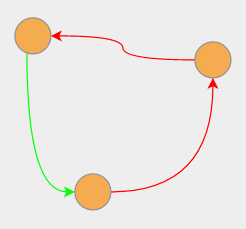
\includegraphics[width=\textwidth]{img/graph-example1-1.png}
				\caption{Original graph}
				\label{fig:img/graph-example1-1.png}
			\end{subfigure}
			\begin{subfigure}[b]{0.3\textwidth}
				\centering
				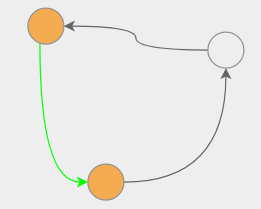
\includegraphics[width=\textwidth]{img/graph-example1-2.png}
				\caption{Integer solution}
				\label{fig:img/graph-example1-2.png}
			\end{subfigure}
			\begin{subfigure}[b]{0.3\textwidth}
				\centering
				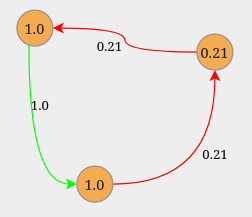
\includegraphics[width=\textwidth]{img/graph-example1-3.png}
				\caption{Relaxed solution}
				\label{fig:img/graph-example1-3.png}
			\end{subfigure}
		\end{center}
		\caption{Model solution for a graph with a single thread, for $\alpha =
				0.3$}
	\end{figure}

\end{frame}

\begin{frame}[c]
	\frametitle{Computing exactly the score - relaxation example}
	\begin{figure}
		\begin{center}
			\begin{subfigure}[b]{0.3\textwidth}
				\centering
				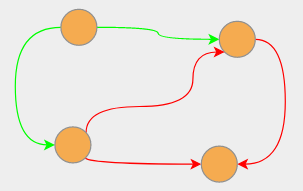
\includegraphics[width=\textwidth]{img/graph-example2-1.png}
				\caption{Original graph}
				\label{fig:img/graph-example2-1.png}
			\end{subfigure}
			\begin{subfigure}[b]{0.3\textwidth}
				\centering
				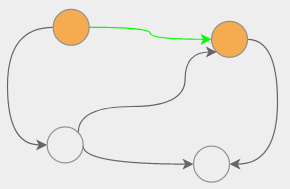
\includegraphics[width=\textwidth]{img/graph-example2-2.png}
				\caption{Integer solution}
				\label{fig:img/graph-example2-2.png}
			\end{subfigure}
			\begin{subfigure}[b]{0.3\textwidth}
				\centering
				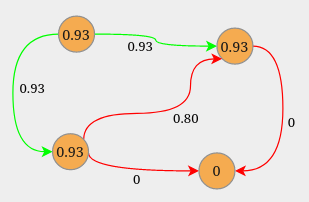
\includegraphics[width=\textwidth]{img/graph-example2-3.png}
				\caption{Relaxed solution}
				\label{fig:img/graph-example1-3.png}
			\end{subfigure}
		\end{center}
		\caption{Model solution for a graph with a single thread, for $\alpha =
				0.3$}
	\end{figure}

\end{frame}

\begin{frame}[c]
	\frametitle{Computing exactly the score - relaxation example}
	\begin{figure}
		\begin{center}
			\begin{subfigure}[b]{0.3\textwidth}
				\centering
				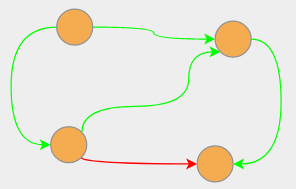
\includegraphics[width=\textwidth]{img/graph-example3-1.png}
				\caption{Original graph}
				\label{fig:img/graph-example3-1.png}
			\end{subfigure}
			\begin{subfigure}[b]{0.3\textwidth}
				\centering
				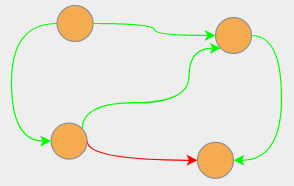
\includegraphics[width=\textwidth]{img/graph-example3-2.png}
				\caption{Integer solution}
				\label{fig:img/graph-example3-2.png}
			\end{subfigure}
			\begin{subfigure}[b]{0.3\textwidth}
				\centering
				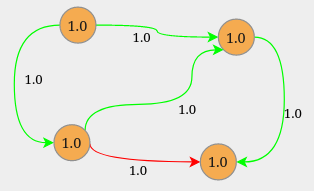
\includegraphics[width=\textwidth]{img/graph-example3-3.png}
				\caption{Relaxed solution}
				\label{fig:img/graph-example3-3.png}
			\end{subfigure}
		\end{center}
		\caption{Model solution for a graph with a single thread, for $\alpha =
				0.3$}
	\end{figure}

\end{frame}

\begin{frame}[c]
	\frametitle{Computing exactly the score - relaxation example}
	\begin{figure}
		\begin{center}
			\begin{subfigure}[b]{0.3\textwidth}
				\centering
				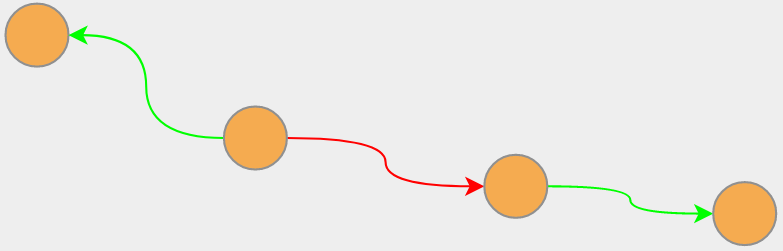
\includegraphics[width=\textwidth]{img/graph-example4-1.png}
				\caption{Original graph}
				\label{fig:img/graph-example4-1.png}
			\end{subfigure}
			\begin{subfigure}[b]{0.3\textwidth}
				\centering
				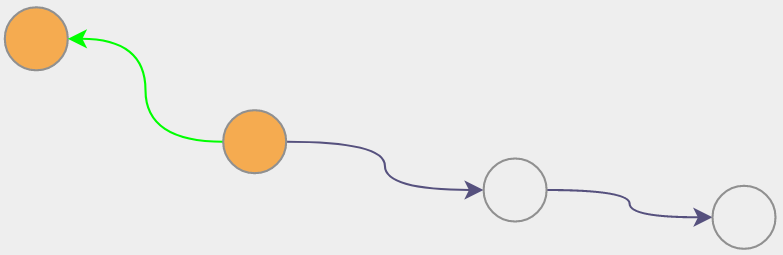
\includegraphics[width=\textwidth]{img/graph-example4-2.png}
				\caption{Integer solution}
				\label{fig:img/graph-example4-2.png}
			\end{subfigure}
			\begin{subfigure}[b]{0.3\textwidth}
				\centering
				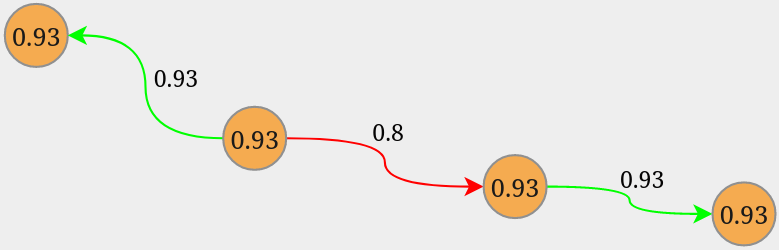
\includegraphics[width=\textwidth]{img/graph-example4-3.png}
				\caption{Relaxed solution}
				\label{fig:img/graph-example4-3.png}
			\end{subfigure}
		\end{center}
		\caption{Model solution for a graph with a single thread, for $\alpha =
				0.3$}
	\end{figure}

\end{frame}

\begin{frame}[c]
	\frametitle{Reconstructing solutions from relaxation results}
	Let

	\begin{equation*}
		U(r) \coloneqq \{ i \in V \; s.t. \; y_i \geq r\}
	\end{equation*}
	\begin{equation*}
		E(r) \coloneqq \{ ij \in E \; s.t. \; x_{ij} \geq r\}
	\end{equation*}
	\begin{equation*}
		\tilde{R} \coloneqq \{ x_{ij} \; \forall ij \in E \}
	\end{equation*}
	\begin{algorithm}[H]
		\SetAlgoLined
		\ForEach{ $r \in \tilde{R}$ }{
			\While {$(V(r), E(r)) \neq T[V(r)]$} {
				remove a vertex that misses one or more edges from $V(r)$ and its
				corresponding edges from $E(r)$\;
			}

			Calculate $\xi({V(r)})$
		}
		\caption{Relaxation results reconstruction}
	\end{algorithm}

\end{frame}

\begin{frame}[c]
	\frametitle{Evaluating echo chamber}
	Results of graph $G$ can be evaluated against random shuffling of the graph
	$G_{r} $.

	\bigskip
	Similarly to \cite{Aref_2018}, signs are allocated randomly on the same
	underlying structure while keeping the same fraction of negative edges.
	This is done separately for each thread.

	\bigskip
	Let $\xi(G_{r} )$ and $\sigma(G_{r} ) $ be the average and standard deviation of
	$\xi$ across the many $G_{r} $, respectively.

	They use Z-score

	\begin{equation}
		Z = \frac{\xi(G) - \xi(G_{r} )}{\sigma(G_{r} ) }
	\end{equation}


\end{frame}


\begin{frame}[c]
	\frametitle{Bibliography}
	\printbibliography
\end{frame}
\end{document}
